% Quantum many-body physics term paper
% Created 03/29/19 by A.T. (tropiano.4@osu.edu)

\documentclass{article}

% Packages
\usepackage{amsmath}
\usepackage{amsfonts}
\usepackage{amssymb}
\usepackage{bm}
\usepackage[font=small,skip=0pt]{caption}
\usepackage{cellspace}
\usepackage{color}
\usepackage{enumerate}
\usepackage{epsfig}
\usepackage[figuresright]{rotating}
\usepackage{float}
\usepackage{graphicx}
\graphicspath{{Figures/}} % Setting the graphics path
\usepackage{hyperref} % For clickable links to sections within table of contents
\usepackage{indentfirst}
\usepackage{physics} % For bra-ket notation
\usepackage{simplewick} % For contractions
\usepackage{siunitx}
\usepackage{subfigure} % For figures with multiple images or pdf's


\begin{document}


%%%%%%%%%%%%%%%%%%%%%%%%%%%%%%%%%%%%%%%%%%%%%%%%%%%%%%%%%%%%%%%%%%%%%%%%%
\title{The nuclear many-body problem and the in-medium similarity renormalization group}


\author{Anthony Tropiano}

\date{\today}

\maketitle


%%%%%%%%%%%%%%%%%%%%%%%%%%%%%%%%%%%%%%%%%%%%%%%%%%%%%%%%%%%%%%%%%%%%%%%%%
\section{Introduction}
\label{sec:intro}


Low-energy nuclear physics addresses the structure and reactions of atomic nuclei. A current area of interest experimentally targets the properties and limits of stability for different isotopes (nuclei with a fixed number of protons and varying number of neutrons). Rare isotope science connects several areas of physics. In nuclear astrophysics, low-energy nuclear reactions can provide insight on the origin of heavy elements in the universe. From the sub-atomic physics standpoint, we can understand fundamental symmetries and interactions from the interplay of the strong, electromagnetic, and weak interactions in atomic nuclei giving rise to physics beyond the Standard Model. Furthermore, rare isotopes have many practical applications in areas outside of physics; for instance, medicinal sciences, material science, and national security. New rare isotope beam facilities have greatly increased our understanding of these areas.
\\

Solving the nuclear many-body problem is the central task for nuclear structure and reactions. The problem at hand is solving a system of protons and neutrons interacting via the strong force. Progress in theoretical nuclear physics has long been impeded by highly correlated many-body wave functions and highly non-perturbative few- and many-body systems. However, there has been substantial headway in the past decade due to effective field theory (EFT) \cite{Epelbaum:2008ga} and renormalization group (RG) methods combined with computational power. We will focus on the theoretical side of low-energy nuclear physics - in particular, the in-medium similarity renormalization group (IMSRG).
\\

A preliminary step in the nuclear many-body problem is to choose efficient degrees of freedom. Quantum chromodynamics (QCD) is widely accepted as the correct underlying theory for the strong interaction; however, it is not an efficient method of calculating nuclei. With EFT we can choose colorless hadron degrees of freedom instead where the properties of nuclei are manifested by interacting protons and neutrons instead of quarks and gluons. This picture is still complicated by high-energy degrees of freedom making many-body methods difficult or even impossible for medium mass and heavier nuclei. With RG methods we can decouple the low- and high-energy degrees of freedom while still preserving the low-energy observables. First, we give a brief description of an EFT called Chiral EFT. Chiral EFT applies chiral perturbation theory to nuclear systems and gives an EFT involving nucleons (N) and Goldstone bosons, which are pions, due to chiral symmetry breaking. This theory is split into long- and short-range terms where the long-range terms (pion exchanges) are calculated explicitly, and the short-range terms (contact terms) are parametrized by NN scattering data. This provides a clear separation of energy scales in the underlying interaction. RG methods allow us to decouple these energy scales while still preserving the low-energy properties of the initial nuclear potential. These are called ``softened'' potentials and serve as inputs to nuclear many-body calculations. This process is considered an \textit{ab initio} method which essentially means making predictions for A-body nuclei starting from microscopic NN and 3N forces. In Fig.~\ref{fig:nuclear_hockey_stick} we see the tremendous progress \textit{ab initio} methods have made in the past decade where each point on the scatter plot corresponds to a binding energy \textit{ab initio} calculation for an A-body nucleus where A is the total number of nucleons.
\\

%
\begin{figure}
  \captionsetup{singlelinecheck=false,justification=raggedright}
  \centering
  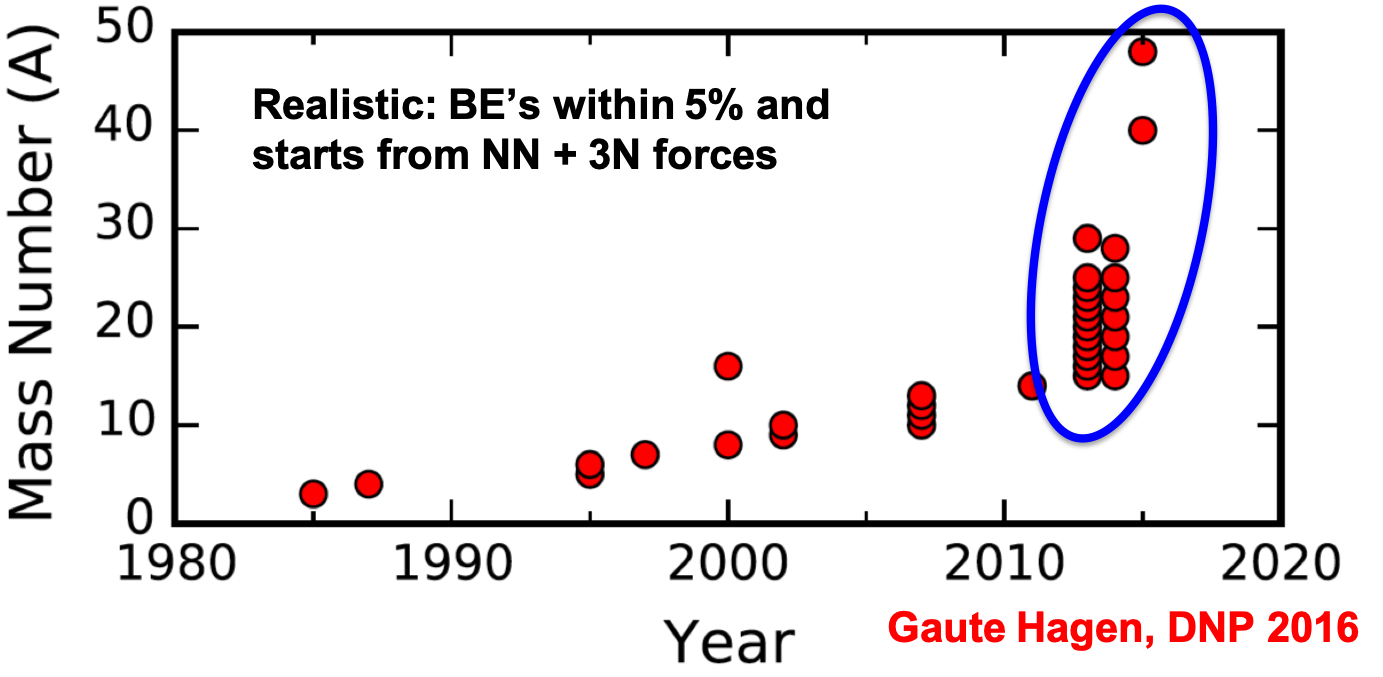
\includegraphics[width=10cm]{nuclear_hockey_stick}
  \caption{Binding energies for A-body nuclei within 5\% of the experimental value calculated from \textit{ab initio} methods.}
  \label{fig:nuclear_hockey_stick}
\end{figure}
%

In the SRG procedure, one applies a unitary transformation to an operator to decouple energy scales \cite{Bogner:2006pc, Bogner:2009bt}. For instance, consider an NN potential in momentum-space; it is useful to think of the potential as a matrix $V(\bf{k},\bf{k'})$ dependent on two momenta $\bf{k}$ and $\bf{k'}$. It is common to express nuclear potentials as a function of the magnitudes $k$ and $k'$ via a partial wave expansion. In momentum-space, the coupling of low- and high-momenta means that $V(k,k')$ has non-zero off-diagonal matrix elements. Applying an SRG transformation to $V(k,k')$ renders the potential as band- or block-diagonal form where the off-diagonal matrix elements are driven zero. One can then truncate the matrix keeping the low-momentum part and still calculate low-energy observables to high accuracy.
\\


The in-medium SRG works in the same manner but targets nuclear Hamiltonians in second quantized form, that is, in Fock-space, and solves the A-body problem directly \cite{Hergert:2015awm, Hergert:2016iju}. Now we can imagine a Hamiltonian matrix that couples some reference state to particle-hole excitations. One must choose a basis and reference state for the system. Typically, we take a harmonic oscillator (HO) configuration-space to describe the single-particle states of protons and neutrons in an A-body nucleus. The low-lying spectrum of the system is dominated by particle-hole excitations near the Fermi level. Thus, a single Slater determinant near the nucleus' ground-state is usually taken as the reference state. An IMSRG transformation decouples the reference state from particle-hole excitations, and in the same way as before, we can obtain all low-energy observables with the decoupled reference state. Fig.~\ref{fig:imsrg_decoupling} depicts this process where the reference state 0p0h is decoupled from particle-hole excitations on the right-hand side. Since the model space can be extremely large, the evolved Hamiltonian is truncated to include only the low-lying space and is used to directly tackle the nuclear many-body problem.
\\

%
\begin{figure}
  \captionsetup{singlelinecheck=false,justification=raggedright}
  \centering
  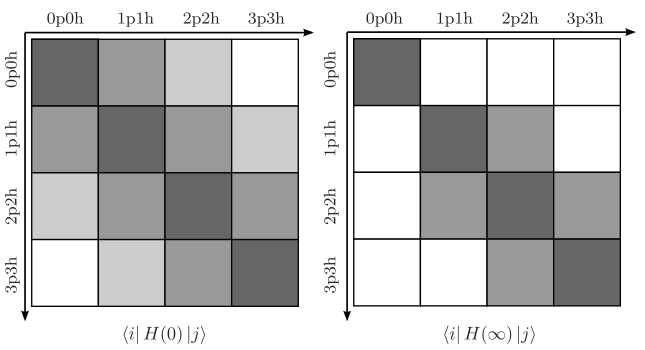
\includegraphics[width=10cm]{imsrg_decoupling}
  \caption{Schematic representation of a nuclear Hamiltonian in Fock-space initially (left) and IMSRG evolved (right) where 0p0h, 1p1h, 2p2h, ... means zero, one, and two particle-hole excitations and so forth with respect to the reference state. White squares correspond to matrix elements equal to zero. (Figure from H. Hergert.)}
  \label{fig:imsrg_decoupling}
\end{figure}
%

The remainder of this paper is organized as follows: Section \ref{sec:formalism} presents the mathematical background of the IMSRG and the formulation in Fock-space in the context of transforming a nuclear Hamiltonian. In Section \ref{sec:applications} we give some results from IMSRG calculations and discuss applications of the IMSRG including effective Hamiltonians, the Magnus expansion, and operator evolution. Lastly, we summarize in Section \ref{sec:conclusion}.


%%%%%%%%%%%%%%%%%%%%%%%%%%%%%%%%%%%%%%%%%%%%%%%%%%%%%%%%%%%%%%%%%%%%%%%%%
\section{Formalism}
\label{sec:formalism}


% .....................................................................................................................................................................................................................................
\subsection{Preliminaries}


The SRG decouples operators by applying a continuous unitary transformation $U(s)$ where $s=0 \rightarrow \infty$ is the flow parameter; that is,
%
\begin{eqnarray}
  \label{eq:srg_hamiltonian}
  H(s) = U(s) H(0) U^{\dagger}(s),
\end{eqnarray}
%
where $H(0)$ corresponds to the `bare' Hamiltonian and $H(s)$ corresponds to the evolved, decoupled Hamiltonian at $s>0$. In practice, the unitary transformation $U(s)$ is not explicitly solved for; the evolved Hamiltonian is given by a differential flow equation. To see this, we take the derivative of Eq.~\ref{eq:srg_hamiltonian},
%
\begin{eqnarray}
  \label{eq:hamiltonian_derivative_1}
  \frac{dH(s)}{ds} = \frac{dU(s)}{ds} H(0) U^{\dagger}(s) + U(s) H(0) \frac{dU^{\dagger}(s)}{ds}.
\end{eqnarray}
%
Rearranging Eq.~(\ref{eq:srg_hamiltonian}) for $H(0)$ and substituting into Eq.~(\ref{eq:hamiltonian_derivative_1}) gives
%
\begin{eqnarray}
  \label{eq:hamiltonian_derivative_2}
  \frac{dH(s)}{ds} = \frac{dU(s)}{ds} U^{\dagger}(s) H(s) + H(s) U(s) \frac{dU^{\dagger}(s)}{ds}.
\end{eqnarray}
%
Because $U(s)$ is unitary, we see that
%
\begin{eqnarray}
  \label{eq:antihermitian_transformation}
  \frac{d}{ds} (U(s) U^{\dagger}(s)) = \frac{d}{ds} (I) = 0 \implies \frac{dU(s)}{ds} U^{\dagger}(s) = -U(s) \frac{dU^{\dagger}(s)}{ds}.
\end{eqnarray}
%
The anti-hermitian SRG generator $\eta(s)$ is defined below in terms of the unitary transformation and its derivative,
%
\begin{eqnarray}
  \label{eq:eta}
  \eta(s) \equiv \frac{dU(s)}{ds} U^{\dagger}(s) = -\eta^{\dagger}(s).
\end{eqnarray}
%
We can now write a concise flow equation for $H(s)$ in terms of the SRG generator $\eta(s)$ by substituting Eq.~(\ref{eq:eta}) into Eq.~(\ref{eq:hamiltonian_derivative_2}),
%
\begin{eqnarray}
  \label{eq:srg_flow}
  \frac{dH(s)}{ds} = [ \eta(s), H(s) ].
\end{eqnarray}
%
We can specify the type of flow for the transformation by choosing $G$ in the equation below,
%
\begin{eqnarray}
  \label{eq:srg_generator}
  \eta(s) = [ G, H(s) ].
\end{eqnarray}
%
For instance, to evolve the Hamiltonian to a band-diagonal form, one can set $G=H_{D}(s)$ (the diagonal of the evolving Hamiltonian), also known as the ``Wegner" generator originally implemented in condensed matter physics \cite{Wegner:1994ab}. Another option is the block-diagonal generator which separates the evolved Hamiltonian into low- and high-momentum sub-blocks \cite{Anderson:2008mu}. For the IMSRG, we must formulate the flow equation (\ref{eq:srg_flow}) and Hamiltonian in the language of second quantization.


% .....................................................................................................................................................................................................................................
\subsection{Normal-ordered A-body Hamiltonian}


Since we are dealing with fermions, consider the fermionic creation and annihilation operators, $a_i^\dagger$ and $a_i$, with the anti-commutation relations
%
\begin{eqnarray}
  \label{eq:fermionic_anticommutators}
  \{ a_i^\dagger, a_j^\dagger \} = \{ a_i, a_j \} = 0, \quad \{ a_i^\dagger, a_j \} = \delta_{ij},
\end{eqnarray}
%
where the indices label single-particle quantum states. We can build a many-body basis by acting the creation operator on the vacuum state,
%
\begin{eqnarray}
  \label{eq:manybody_basis}
  \ket{\Phi(i_1, ... \, , i_A)} = \prod_{k=1}^{A} a_{i_k}^\dagger \ket{0}.
\end{eqnarray}
%
As mentioned before, it is much more efficient to work with a reference state near the Fermi level for construction and organization of the many-body basis. Therefore, we take a reference state $\ket{\Phi}$ near the ground-state of the A-body nucleus. We introduce a one-body operator that is normal-ordered with respect to the reference state below,
% 
\begin{eqnarray}
  \label{eq:normal_ordering}
  a_i^\dagger a_j \equiv \, : \! a_i^\dagger a_j \! : + \contraction{}{a}{_i^\dagger}{a} a_i^\dagger a_j,
\end{eqnarray}
%
where the $: \! ... \! :$ indicates normal-ordering and the brace over $a_i^\dagger$ and $a_j$ means they have been contracted. A contraction is the expectation value of the operator in the reference state $\ket{\Phi}$:
%
\begin{eqnarray}
  \label{wick_contraction}
  \contraction{}{a}{_i^\dagger}{a} a_i^\dagger a_j \equiv \mel{\Phi}{a^\dagger_i a_j}{\Phi} \equiv \rho_{ji}.
\end{eqnarray}
%
We can now write any A-body operator as a normal-ordered operator by evaluating contractions between creation and annihilation operators. 
\\


Because nuclei are self-bound objects and therefore translationally invariant, we only need to consider nucleon momenta relative to the center of mass in writing the total kinetic energy. Thus, we consider an intrinsic Hamiltonian where the center of mass kinetic energy is subtracted out: $T_{int} = T - T_{cm}$. We refer to $T_{int}$ as $T$ in the rest of the paper. Then an A-body Hamiltonian with both NN and 3N interactions can be written as,
%
\begin{eqnarray}
  \label{eq:intrinsic_hamiltonian}
  H = (1-\frac{1}{A}) T^{(1)} + \frac{1}{A} T^{(2)} + V^{(2)} + V^{(3)},
\end{eqnarray}
%
where the one- and two-body kinetic energy terms are
%
\begin{eqnarray}
  \label{eq:one_body_kinetic_energy}
  T^{(1)} = \sum_i \frac{ \textbf{p}_i^2 }{ 2m },
\end{eqnarray}
%
\begin{eqnarray}
  \label{eq:one_body_kinetic_energy}
  T^{(2)} = - \frac{1}{m} \sum_{i<j} \textbf{p}_i \cdot \textbf{p}_j.
\end{eqnarray}
%
Note, the sum of the one- and two-body kinetic energy terms are equivalent to a kinetic energy term, $T = \frac{2}{A } \sum_{i<j} \frac{ \textbf{q}_{ij}^2 }{ 2 \mu }$, where $\textbf{q}_{ij}$ is the momentum transfer between two nucleons and $\mu$ is the reduced mass \cite{Hergert:2009na}. Now we can write the Hamiltonian in terms of normal-ordered zero-, one-, two-, and three-body terms where the labels have been chosen for historical reasons,
%
\begin{eqnarray}
  \label{eq:exact_hamiltonian}
  H &=& E + \sum_{ij} f_{ij} : \! a_i^\dagger a_j \! : + \frac{1}{4} \sum_{ijkl} \Gamma_{ijkl} : \! a_i^\dagger a_j^\dagger a_l a_k \! : \nonumber \\
& & + \frac{1}{36} \sum_{ijklmn} W_{ijklmn} : \! a_i^\dagger a_j^\dagger a_k^\dagger a_n a_m a_l \! :.
\end{eqnarray}
%
It is convenient to work in the eigenbasis of the one-body density matrix in defining each contribution in Eq.~(\ref{eq:exact_hamiltonian}), such that
%
\begin{eqnarray}
  \label{eq:one_body_density_matrix}
  \rho_{ab} = n_a \delta_{ab}, \quad n_a \in \{ 0, 1 \}.
\end{eqnarray}
%
Then the normal-ordered terms are given by the following:
%
\begin{eqnarray}
  \label{eq:zero_body_hamiltonian}
  E &=& (1-\frac{1}{A}) \sum_a \mel{a}{T^{(1)}}{a} n_a + \frac{1}{2} \sum_{ab} \mel{ab}{ \frac{1}{A} T^{(2)} + V^{(2)} }{ab} n_a n_b \nonumber \\ 
& & + \frac{1}{6} \sum_{abc} \mel{abc}{V^{(3)}}{abc} n_a n_b n_c,
\end{eqnarray}
%
\begin{eqnarray}
  \label{eq:one_body_hamiltonian}
  f_{ij} &=& (1-\frac{1}{A}) \mel{i}{T^{(1)}}{j} + \sum_{a} \mel{ia}{ \frac{1}{A} T^{(2)} + V^{(2)} }{ja} n_a \nonumber \\
& & + \frac{1}{2} \sum_{ab} \mel{iab}{V^{(3)}}{jab} n_a n_b,
\end{eqnarray}
%
\begin{eqnarray}
  \label{eq:two_body_hamiltonian}
  \Gamma_{ijkl} = \mel{ij}{ \frac{1}{A} T^{(2)} + V^{(2)} }{kl} + \sum_{a} \mel{ija}{V^{(3)}}{kla} n_a,
\end{eqnarray}
%
\begin{eqnarray}
  \label{eq:three_body_hamiltonian}
  W_{ijklmn} = \mel{ijk}{V^{(3)}}{lmn}.
\end{eqnarray}
%
Due to the occupation numbers in Eqs.~(\ref{eq:zero_body_hamiltonian})-(\ref{eq:two_body_hamiltonian}), the sums run over only hole states leading to a 3N contribution in each term.


% .....................................................................................................................................................................................................................................
\subsection{IMSRG flow equations}


When carried out exactly, the evaluation of the commutator on the RHS of Eq.~(\ref{eq:srg_flow}) induces higher-body interactions, implying that $H(s)$ and $\eta(s)$ are A-body operators despite starting out with a lower particle rank at $s=0$. This is seen by considering the following commutator and applying Wick's theorem to evaluate the product of normal-ordered operators,
%
\begin{eqnarray}
  \label{eq:induced_forces}
  [ \, : \! a_i^\dagger a_j^\dagger a_l a_k \! :, \, :a_p^\dagger a_q^\dagger a_s a_r \! : \, ] = \delta_{kp} : \! a_i^\dagger a_j^\dagger a_q^\dagger a_s a_r a_l \! : + \, ...
\end{eqnarray}
%
Hence, every integration step in the flow equation contributes an induced, higher-body term to $H(s)$. Keeping all induced terms is not numerically feasible and a truncation scheme must be introduced. We will consider a simple truncation scheme in which three-body and higher normal-ordered terms in $H(s)$ and $\eta(s)$ are excluded. That is,
%
\begin{eqnarray}
  \label{eq:imsrg2_hamiltonian}
  H(s) \approx E(s) + f(s) + \Gamma(s),
\end{eqnarray}
%
\begin{eqnarray}
  \label{eq:imsrg2_eta}
  \eta(s) \approx \eta^{(1)}(s) + \eta^{(2)}(s).
\end{eqnarray}
%
This is called the IMSRG(2) truncation. Now we can write the IMSRG(2) flow equations in terms of the normal-ordered contributions. Define the permutation symbol as
%
\begin{eqnarray}
  \label{eq:permutation_symbol}
  P_{ij} g(... \, , i, ... \, , j) \equiv g(... \, , j, ... \, , i).
\end{eqnarray}
%
Then the IMSRG(2) flow equations can be written as
%
\begin{eqnarray}
  \label{imsrg_flow_zero_body}
  \frac{dE}{ds} = \sum_{ab} (n_a - n_b) \eta_{ab} f_{ba} + \frac{1}{2} \sum_{abcd} \eta_{abcd} \Gamma_{cdab} n_a n_b \bar{n}_c \bar{n}_d ,
\end{eqnarray}
%
\begin{eqnarray}
  \label{imsrg_flow_one_body}
  \frac{df_{ij}}{ds} &=& \sum_a (1+P_{ij}) \eta_{ia} f_{aj} + \sum_{ab} (n_a-n_b) ( \eta_{ab} \Gamma_{biaj} - f_{ab} \eta_{biaj} ) \nonumber \\
& & + \frac{1}{2} \sum_{abc} ( n_a n_b \bar{n}_c + \bar{n}_a \bar{n}_b n_c ) (1+P_{ij}) \eta_{ciab} \Gamma_{abcj},
\end{eqnarray}
%
\begin{eqnarray}
  \label{imsrg_flow_two_body}
  \frac{d\Gamma_{ijkl}}{ds} &=& \sum_{a} \{ (1-P_{ij})( \eta_{ia} \Gamma_{ajkl} - f_{ia} \eta_{ajkl} ) - (1-P_{kl})( \eta_{ak} \Gamma_{ijal} - f_{ak} \eta_{ijal} ) \} \nonumber \\ 
& & + \frac{1}{2} \sum_{ab} (1-n_a-n_b) ( \eta_{ijab} \Gamma_{abkl} - \Gamma_{ijab} \eta_{abkl} ) \nonumber \\
& & + \sum_{ab} (n_a-n_b)(1-P_{ij})(1-P_{kl}) \eta_{aibk} \Gamma_{bjal},
\end{eqnarray}
%
where $\bar{n}_i = 1 - n_i$. By integrating the IMSRG flow equations, we can decouple an A-body nuclear Hamiltonian and obtain low-energy observables.
\\


The previous description of the IMSRG flow equations are referred to as the M-scheme flow equations. An extension of this, called the J-scheme flow equations, is designed for spherically symmetric systems. We take a spherically symmetric reference state and preserve rotational symmetry in every term of the nuclear Hamiltonian. Then the flow equations become block-diagonal in angular momentum and independent of angular momentum projection quantum numbers. Implementing the J-scheme flow equations greatly reduces the computational cost of evolving the Hamiltonian.


%%%%%%%%%%%%%%%%%%%%%%%%%%%%%%%%%%%%%%%%%%%%%%%%%%%%%%%%%%%%%%%%%%%%%%%%%
\section{Applications}
\label{sec:applications}


% .....................................................................................................................................................................................................................................
\subsection{Example calculations}


A number of IMSRG example calculations and applications are presented in the following sections. First, we explore how decoupling of a nuclear Hamiltonian works in practice. In Fig.~\ref{fig:imsrg_40Ca_decoupling} we show matrix elements of $^{40}$Ca in the $J^{\pi}=0^+$ neutron-neutron interaction for several different values of $s$. The notation $J^{\pi}=0^+$ means the total angular momentum of the two nucleons is zero with parity +1. The evolution of the Hamiltonian is carried out by integrating the IMSRG(2) J-scheme flow equations with a high-order ODE solver. The input interaction is a chiral NN potential softened by SRG evolution. We see that as $s$ is taken to higher values, the off-diagonal $hhpp$ and $pphh$ matrix elements are driven to zero, that is, $\Gamma_{pp'hh'}(s)$ becomes small as desired.
\\

%
\begin{figure}
  \captionsetup{singlelinecheck=false,justification=raggedright}
  \centering
  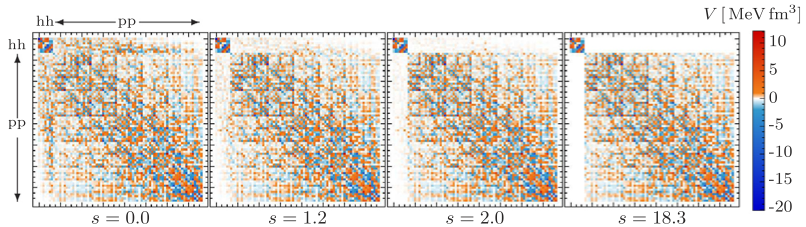
\includegraphics[width=12cm]{imsrg_40Ca_decoupling}
  \caption{Matrix elements of $^{40}$Ca in the $J^{\pi}=0^+$ neutron-neutron interaction for IMSRG(2) evolutions of $s=0.0$, $1.2$, $2.0$, and $18.3$. Only the hhhh, hhpp, pphh, and pppp sub-blocks of the matrix are shown. (Figure from \cite{Hergert:2015awm}.)}
  \label{fig:imsrg_40Ca_decoupling}
\end{figure}
%

We show IMSRG predictions for ground-state energies of several nuclei. Figure \ref{fig:imsrg_gs_energies} shows IMSRG ground-state energies for $^{78}$Ni, $^{100}$Sn, and $^{132}$Sn with respect to $\hbar \omega$ and single-particle basis size $e_{max}$. These calculations were done using the IMSRG(2) J-scheme with the same NN interaction as before. The gray-dashed line is the found by extrapolating $e_{max} \geq 10$ data sets to infinite basis size. We see a convergence pattern for increasing basis size $e_{max}$ and $\hbar \omega$ in each panel. Overall, the convergent ground-state energies are consistent with other many-body methods such as the No-Core Shell Model or Coupled Cluster methods.
\\


All of the nuclei presented so far are closed-shell nuclei, that is, the occupation orbitals in the nuclear shell model are all filled similar to filled electron orbitals for a noble gas. An open-shell nuclei is a system with valence nucleons occupying states outside an inert core. The following section discusses a method that allows the IMSRG to target open-shell nuclei.
\\

%
\begin{figure}
  \captionsetup{singlelinecheck=false,justification=raggedright}
  \centering
  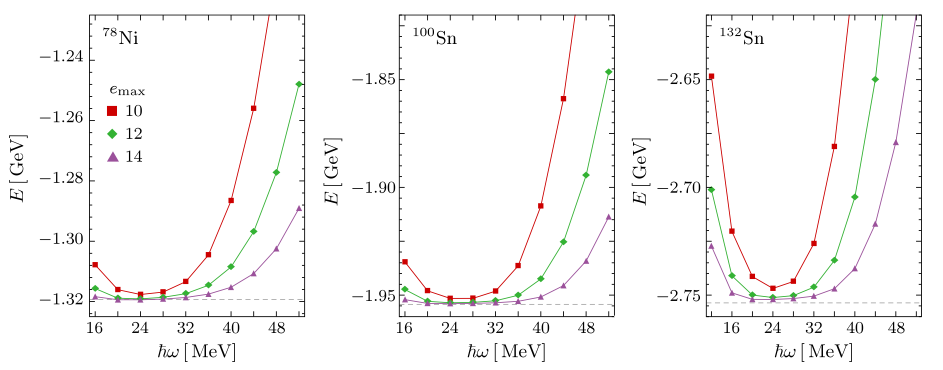
\includegraphics[width=12cm]{imsrg_gs_energies}
  \caption{Convergence of ground-state energies for $^{78}$Ni, $^{100}$Sn, and $^{132}$Sn using IMSRG(2). (Figure from \cite{Hergert:2015awm}.)}
  \label{fig:imsrg_gs_energies}
\end{figure}
%


% .....................................................................................................................................................................................................................................
\subsection{Effective Hamiltonians}


We can target open-shell nuclei by splitting up the single-particle basis into three parts: hole states (h), valence states (v), and non-valence (q) states. We take our reference state $\ket{\Phi}$ as the wave function of the inert core, which can be obtained from a spherical Hartree-Fock (HF) calculation. That is, the nuclear Hamiltonian is normal-ordered with respect to the inert core. Then following the nuclear shell model, we can build an effective Hamiltonian where nucleons in the valence states serve as the degrees of freedom (called valence nucleons). This process can be done microscopically using many-body perturbation theory (MBPT); however, the order-by-order convergence is unclear and results are sensitive to the configuration-space details (HO frequency, choice of valence-space, etc.)
\\


The IMSRG can derive effective valence-space Hamiltonians by decoupling the reference state from valence states. Furthermore, we can decouple valence states (v) from non-valence states (q). Then by diagonalizing the effective Hamiltonian, we can predict the ground-state energy and low-lying excited states. This method is commonly referred to as valence-space IMSRG (VS-IMSRG). In Fig.~\ref{fig:imsrg_O_energy_spectra} we show a comparison of VS-IMSRG calculations to other methods and experimental data for oxygen excitation energies. Gysbers \textit{et al.}~\cite{Gysbers:2019uyb} recently showed significant improvement in nuclear $\beta$-decay calculations using the VS-IMSRG method with consistently evolved operators over the phenomenological shell model approach.

%
\begin{figure}
  \captionsetup{singlelinecheck=false,justification=raggedright}
  \centering
  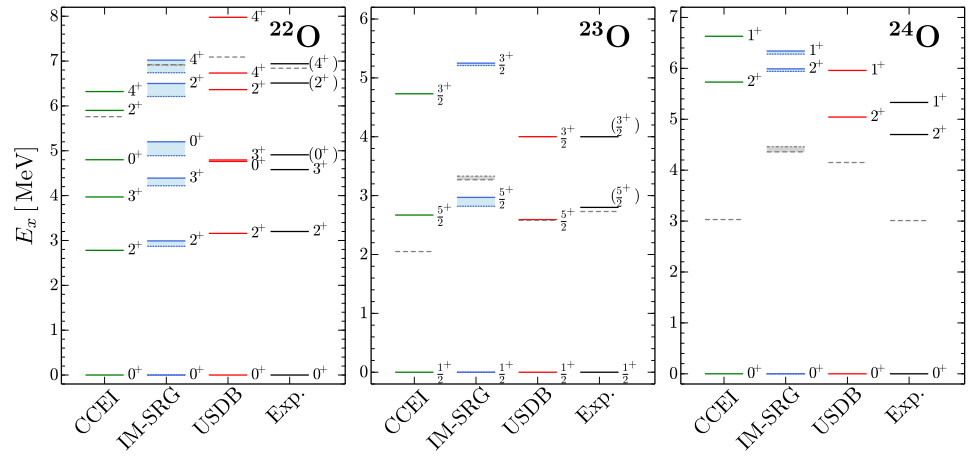
\includegraphics[width=12cm]{imsrg_O_energy_spectra}
  \caption{Excitation spectra of oxygen isotopes using effective interactions derived by VS-IMSRG decoupling (blue solid and dashed lines where the shaded band represents varying $\hbar \omega$ from 20-24 MeV), the coupled-cluster effective interaction (CCEI) approach (green lines), and phenomenological USDB interaction (red lines) in comparison to experimental data (black lines). The dashed lines represent the neutron separation energies. (Figure from \cite{Hergert:2016etg}.)}
  \label{fig:imsrg_O_energy_spectra}
\end{figure}
%


% .....................................................................................................................................................................................................................................
\subsection{The Magnus expansion}


The IMSRG procedure requires solving a system of nonlinear, coupled differential equations which can often be stiff, necessitating a high-order ODE solver. In principle, the evolved Hamiltonian (or any operator) is unitarily equivalent but the numerical error of solving the ODE can lead to error on observable quantities. Furthermore, the model spaces for IMSRG calculations can be extremely large. Evolving several operators is often impossible due to computational memory restrictions in storing several operators. A variant of the IMSRG that utilizes a mathematical technique called the Magnus expansion can overcome these limitations \cite{Morris:2015yna}. We will refer to this as the Magnus implementation or simply Magnus.
\\


The Magnus posits that the unitary transformation takes the form $U(s)=e^{\Omega(s)}$ where $\Omega(s)$ is an anti-hermitian matrix. We then solve for $\Omega(s)$ by integrating its formally exact derivative (details are in \cite{Morris:2015yna}) which allows one to construct $U(s)$ explicitly. From the form of the transformation, any numerical error from solving the ODE leaves the unitarity of the evolved Hamiltonian un-affected preserving the observables. In fact, we can apply a first-order ODE method in solving for $\Omega(s)$ and keep the observables intact. This offers a decent computational speed-up by avoiding a high-order solver. In Fig.~\ref{fig:magnus_16O_gs_energy} we show the $^{16}$O ground-state energy evolving with $s$ comparing the typical IMSRG approach and Magnus implementation where a first-order Euler method ODE solver is used for two step-sizes $\delta s$. An IMSRG curve using a high-order solver is included for comparison. We see that the Magnus approaches the high-order IMSRG result despite the crude first-order method whereas the IMSRG suffers from using a first-order solver. This illustrates the advantage of guaranteed unitarity from the Magnus implementation.
\\

%
\begin{figure}
  \captionsetup{singlelinecheck=false,justification=raggedright}
  \centering
  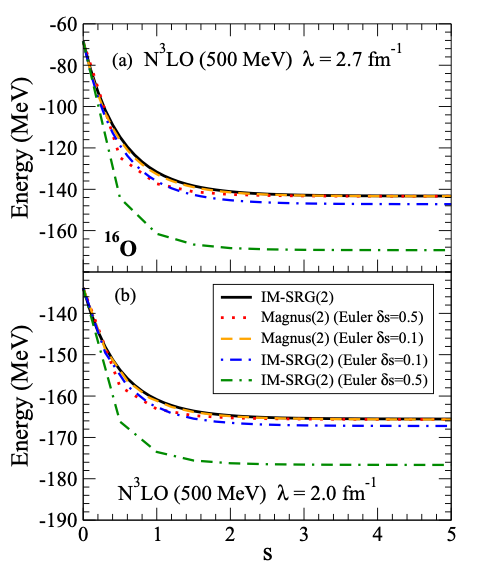
\includegraphics[width=6cm]{magnus_16O_gs_energy}
  \caption{Ground-state energy of $^{16}$O with respect to the flow parameter $s$ for two SRG softened potentials. The black line corresponds to the standard IMSRG(2) method with a high-order ODE solver. The red dotted and yellow dashed lines correspond to the Magnus implementation using the first-order Euler method where $\delta s$ represents the step-size. The blue dash-dotted and green dash-dotted lines correspond to the IMSRG(2) using the first-order Euler method. (Figure from \cite{Morris:2015yna}.)}
  \label{fig:magnus_16O_gs_energy}
\end{figure}
%

By explicitly solving for the transformation, one can evolve several operators. We simply apply $U(s)$ to any bare operator using the Baker-Campbell-Hausdorff (BCH) formula. In the standard procedure, the solution vector in the flow equation would contain the evolving Hamiltonian as well as any additional operator making drastic demands on computational memory. For these reasons, the Magnus implementation has become a standard technique in IMSRG calculations as studies have targeted observables such as radii, electromagnetic moments and transitions, etc., requiring consistently evolved operators \cite{Parzuchowski:2017wcq}.


%%%%%%%%%%%%%%%%%%%%%%%%%%%%%%%%%%%%%%%%%%%%%%%%%%%%%%%%%%%%%%%%%%%%%%%%%
\section{Conclusion}
\label{sec:conclusion}


In summary, we discussed the \textit{ab initio} IMSRG approach to solving the nuclear many-body problem. In the IMSRG method, a reference state for some A-body system is decoupled from higher excitations via a unitary transformation. The decoupled reference state then contains unitarily equivalent low-energy observables solving the A-body problem. We detailed the IMSRG procedure in second quantization following the M-scheme IMSRG(2) method. Closed-shell results show decoupling and convergent ground-state energies. We briefly presented the VS-IMSRG method in which the Hamiltonian is configured in valence-space to serve as an effective Hamiltonian in shell model calculations. Lastly, we introduced the Magnus expansion in the context of the IMSRG and its importance in general operator evolution.
\\


There are several interesting applications of the IMSRG that were not covered in this paper. In many cases, often for open-shell nuclei, the energy gap in the single-particle spectrum is small leading to near-degenerate excited states with respect to the reference state giving strong configuration mixing. The wave function is said to feature collective correlations when configurations involve many nucleons that are excited simultaneously. The multi-reference IMSRG (MR-IMSRG) method accounts for collective correlations in the wave function of the reference state, extending the reach to more diverse systems such as open-shell nuclei . Furthermore, new studies have focused on consistent evolution of operators other than the Hamiltonian. It is important to understand the effects these transformations have on general operators in the sense that we expect induced interactions from the SRG framework. Lastly, since the introduction of the SRG method to nuclear physics, there has been considerable progress in constructing EFT potentials differing in a number of ways. It would be good to revisit SRG evolution of these interactions to gain insight on renormalizability.


%%%%%%%%%%%%%%%%%%%%%%%%%%%%%%%%%%%%%%%%%%%%%%%%%%%%%%%%%%%%%%%%%%%%%%%%%
\begin{thebibliography}{99}


\bibitem{Epelbaum:2008ga}
E.~Epelbaum, H.~-W.~Hammer, and U.~G.~Mei�ner,
Rev. Mod. Phys. {\bf 81}, 1773 (2009) arXiv:0811.1338 [nucl-th].

\bibitem{Bogner:2006pc}
S.~K.~Bogner, R.~J.~Furnstahl, and R.~J.~Perry,
Phys. Rev. C. {\bf 75}, 061001 (2007), arXiv:nucl-th/0609003.

\bibitem{Bogner:2009bt}
S.~K.~Bogner, R.~J.~Furnstahl, and A.~Schwenk,
Prog. Part. Nucl. Phys. {\bf 65}, 94 (2010), arXiv:0912.3688 [nucl-th].

\bibitem{Hergert:2015awm}
H.~Hergert, S.~K.~Bogner, T.~D.~Morris, A.~Schwenk, and K.~Tsukiyama,
Phys. Rept. {\bf 621}, 165 (2016), arXiv:1512.06956 [nucl-th].

\bibitem{Hergert:2016iju}
H.~Hergert, S.~K.~Bogner, J.~G.~Lietz, T.~D.~Morris, S.~Novario, N.~M.~Parzuchowski, and F.~Yuan,
Lect. Notes Phys. {\bf 936}, 477 (2017), arXiv:1612.08315 [nucl-th].

\bibitem{Wegner:1994ab}
F.~Wegner,
Annalen der Physik {\bf 506}, 77 (1994).

\bibitem{Anderson:2008mu}
E.~Anderson, S.~K.~Bogner, R.~J.~Furnstahl, E.~D.~Jurgenson, R.~J.~Perry, and A.~Schwenk,
Phys. Rev. C {\bf 77}, 037001 (2008), arXiv:0801.1098 [nucl-th].

\bibitem{Hergert:2009na}
H.~Hergert, and R.~Roth,
Phys. Lett. B {\bf 682}, 27 (2009), arXiv:0908.1334 [nucl-th].

\bibitem{Gysbers:2019uyb}
P.~Gysbers, \textit{et al.},
Nature Physics, (2019), arXiv:1903.00047 [nucl-th].

\bibitem{Hergert:2016etg}
H.~Hergert,
Phys. Scr. {\bf 92}, 023002 (2017), arXiv:1607.06882 [nucl-th].

\bibitem{Morris:2015yna}
T.~D.~Morris, N.~Parzuchowski, S.~K.~Bogner,
Phys. Rev. C {\bf 92}, 034331 (2015), arXiv:1507.06725 [nucl-th].

\bibitem{Parzuchowski:2017wcq}
N.~M.~Parzuchowski, S.~R.~Stroberg, S.~R.~Navr\'atil, H.~Hergert, and S.~K.~Bogner,
Phys. Rev. C {\bf 96}, 034324 (2017), arXiv:1705.05511 [nucl-th].


\end{thebibliography}


\end{document}